\documentclass[10pt, a4paper]{article}
\clubpenalty1000000
\widowpenalty1000000
\usepackage{lrec2014}
\usepackage{graphicx}
\usepackage[pdfborder={0 0 0}]{hyperref}
\usepackage{listings}
\usepackage{amsmath,amssymb,colortbl,xcolor,color}
\usepackage{tipa}

\usepackage{fontspec}
\newfontfamily\free{FreeSans}
\usepackage{zhspacing}
\zhspacing
\setmainfont{FreeSans}

\title{Concepticon: A Resource for the Linking of Concept Lists}

\name{Johann-Mattis List$^{1}$, Michael Cysouw$^{2}$, Robert Forkel$^{3}$}

\address{ 
               $^{1}$CRLAO/EHESS and AIRE/UPMC, Paris,
	       $^{2}$Forschungszentrum Deutscher Sprachatlas, Marburg,\\
	       $^{3}$Max Planck Institute for the Science of Human History, Jena
	       \\
	       \href{mailto:mattis.list@lingpy.org}{mattis.list@lingpy.org}, 
	       \href{mailto:email}{emailpending}, 
	       \href{mailto:email}{emailpending}\\
	       }


\abstract{
We present an attempt to link the large amount of different concept lists (aka ``Swadesh lists'')
which are used in the linguistic literature. This resource, the \emph{Concepticon}
(\url{http://concepticon.clld.org}), links
\conceptnumber concept labels from \listnumber conceptlists to \setnumber concept sets. Each
concept set is given a unique identifier, a unique label, and a human-readable definition.
Concept sets are further structured by defining different relations between the concepts.  The
resource can be used for various purposes. Serving as a rich reference for new
and existing databases in diachronic and synchronic linguistics, it allows researchers a quick
access to studies on semantic change, cross-linguistic polysemies, and semantic associations. 
\newline \Keywords{concepts, concept lists, Swadesh lists, cross-linguistically linked data}}


% this command serves to get easy access to the basis in hyperref
\newcommand{\concepticon}[1]{http://concepticon.clld.org/contributions/#1}
\newcommand{\conceptnumber}{\textcolor{red}{xxx} }
\newcommand{\listnumber}{\textcolor{red}{xxx} }
\newcommand{\setnumber}{\textcolor{red}{xxx} }
\newcommand{\relationnumber}{\textcolor{red}{xxx} }

\begin{document}

\maketitleabstract

\section{Introduction}
In 1950, Morris Swadesh (1909 -- 1967) proposed the idea that certain parts of the lexicon of human
languages are universal, stable over time, and rather resistant to borrowing. As a result, he
claimed that these
parts of the lexicon, which was later called \emph{basic vocabulary}, would be very
useful to address the problem of subgrouping in historical linguistics:
\begin{quote}
[...] it is a well known fact that certain types of morphemes are relatively stable. Pronouns and
numerals, for example, are occasionally replaced either by other forms from the same language or by
borrowed elements, but such replacement is rare. The same is more or less true of other everyday
expressions connected with concepts and experiences common to all human groups or to the groups
living in a given part of the world during a given epoch. \cite[157]{Swadesh1950}
\end{quote}
He illustrated this by proposing a first \emph{list of basic concepts}, which was, in fact, nothing
else than a collection of concept labels, as shown below:\footnote{This list contains 123 items in
total. According to Swadesh, these items occurred both in his original test list of English items,
and in the data on the Salishan languages, which he employed for his first glottochronological
study.}
\begin{quote}
I, thou, he, we, ye, one, two, three, four, five,
six, seven, eight, nine, ten, hundred, all,
animal, ashes, back, bad, bark, belly, big,
black, blood, bone, brother (elder), child
(son or daughter), cloud, cold, come, cry
(weep), dance, day, dog, dust, ear, earth, eat,
egg, eye, far, father, fire, flower, fog, foot,
good, grass, green, hair, hand, head, heart,
here, hit (with fist), hunt, husband, ice,
lake, laugh, leaf, left hand, leg, liver, long,
louse, man, meat, mother, mountain, mouth,
name, near, neck, night, nose, person, rain,
red, right hand, road (trail), root, rope, salt,
sand, short, sing, sister (elder), skin, sky,
small, smoke, snake, snow, speak, spear
(war), star, stone, sun, swim, tail, that, there,
this, tongue, tooth, tree, warm, water, what,
where, white, who, wife, wind, woman, year,
yellow. \cite[161]{Swadesh1950}
\end{quote}
In the following years, Swadesh refined his original concept lists of basic vocabulary items,
thereby reducing the original test list of 215 items first to 200 \cite{Swadesh1952} and then to 100
items \cite{Swadesh1955}. Scholars working on different language families and different datasets
provided further modifications, be it that the concepts which Swadesh had proposed were lacking
proper translational equivalents in the languages they were working on, or that they
turned out to be not as stable and universal as Swadesh had claimed \cite{Matisoff1978,Alpher1999}. 
Up to today, dozens of different concept list have been compiled for various purposes.
They are are used as heuristical tools for the detection of deep genetic
relationships among languages \cite{Dolgopolsky1964}, 
as basic values for traditional
lexicostatistical and glottochronological studies \cite{Dyen1992,Starostin1991}, 
or as litmus test
for dubious cases of language relationship which might be due to inheritance or borrowing 
\cite{McMahon2005b,Chen1996,Wang2006}. 
 
Apart from concept lists proposed for the application in historical linguistics, there is
a large amount of not explicitly diachronic data, including concept lists serving as the
basis for field work in specific linguistic areas \cite{Kraft1981}, concept lists which serve as the
basis for large surveys on specific linguistic phenomena \cite{Wold2009}, or concept lists which deal with
the internal \emph{structuring} of concepts, be it cognitive associations \cite{Nelson2004},
cross-linguistic polysemies \cite{List2014f}, or frequently recurring semantic shifts
\cite{Bulakh2013}.


\section{Concept Lists}
Concept lists are -- simply speaking -- lists of concepts. In these lists, concepts are ideally
described by a \emph{concept label} and a short \emph{definition}. Most published
concept lists, however, only contain a concept label. On the other hand, certain concept lists have
been further expanded by
adding structure, such as \emph{rankings}, \emph{divisions}, or \emph{relations}.

\subsection{Purpose of Concept Lists}
Concept lists are compiled for a variety of different
purposes. A major distinction can be made between those concept lists which have been compiled for
the
purpose of \emph{language comparison} and those which have been compiled for the purpose of \emph{concept
comparison}. 
Among the former, we can further distinguish those lists which are used to prove \emph{language
relationship} \cite{Dolgopolsky1964}, those which are used for \emph{linguistic subgrouping}
\cite{Norman2003,Starostin1991,Swadesh1955}, and those which can be used to identify \emph{contact
layers} \cite{Chen1996}. Among the latter, we can distinguish between concept lists with a primarily
\emph{synchronic objective} \cite{Hill2014}, and those with a primarily \emph{diachronic objective}
\cite{Wold2009,Bulakh2013}.

\subsection{Structure of Concept Lists}
The purpose for which a given concept list was originally defined has an intermediate influence on
its structure. Given the multitude of use cases in both synchronic and diachronic linguistics, it is
difficult to give an exhaustive and unique classification schema for all concept lists which have
been compiled in the past. In Table \ref{tab:conceptlists}, we have nevertheless tried to
distinguish eight basic types of concept lists and give one list for each of the types as a
prototypical example.\footnote{For further information regarding these concept lists, just click on
the links in the ``Example" field of the table.}

\begin{table}[h]
\resizebox{0.475\textwidth}{!}{%
\tabular{|p{4cm}|p{4cm}|p{4cm}|}
\hline
\bf Type                                & \bf Example                                  & \bf Purpose \\\hline\hline
basic vocabulary list (``Swadesh list") & \href{\concepticon/Swadesh-1952-200}{Swadesh 1952 / 200 items}                     & subgrouping \\\hline
subdivided concept list                 & \href{\concepticon/Yakhontov-1991-100}{Yakhontov 1991 (see
Starostin 1991) / 35 + 65 items}               & genetic relationship, layer identification \\\hline
``ultra-stable" concept list            & \href{\concepticon/Dolgopolsky-1964-15}{Dolgopolsky 1964 /
15 items}                & genetic relationship \\\hline
questionnaire                           & \href{\concepticon/Allen-2007-500}{Allen 2007 / 500
items}                    & dialect / language comparison \\\hline
ranked list                             & \href{\concepticon/Starostin-2007-110}{Starostin 2007 /
110 items}                  & subgrouping, layer identification \\\hline
list of concept relations               & \href{\concepticon/Bulakh-2013-870}{DatSemShift, Bulakh et
al. 2013 / 2424 items} & representation of concept
relations \\\hline
special-purpose concept list            & \href{\concepticon/Matisoff-1978-200}{Matisoff 1978 / 200
items}                 & subgrouping of Tibeto-Burman languages \\\hline
historical concept list                 & \href{\concepticon/Leibniz-1768-128}{Leibniz 1768 / 128
items}                    & language comparison \\\hline
\endtabular}
\caption{Examples for different types of concept list as they can be found in the literature.}
\label{tab:conceptlists}
\end{table}
\nocite{Swadesh1952,Starostin1991,Dolgopolsky1964,Allen2007,Bulakh2013,Matisoff1978,Leibniz1768}

\section{Linking Concept Lists}
\textcolor{red}{+++}While all the concept lists which have been published so far constitute language
resources with rich and valuable information, we lack guidelines, standards, best practices, and
models to handle their interoperability. This is specifically important in the context of
multilingual language resources and resources on less-well-studied languages. 
Language diversity is often addressed with region- or
language-specific questionnaires. This makes it difficult to integrate and compare these resources
on a greater scale. Despite the growing body, the interoperability of language resources involving
concepts and meanings, like wordlists and lexical datasets, has not yet been addressed in a
systematic way.  
 
The Concepticon is an attempt to overcome these difficulties by linking 
the many different concept lists (``Swadesh Lists'') which are
used in the linguistic literature. 
In order to do so, we offer open, linked, and shared data and tools in open and collaborative
architectures. Our data is curated open and collaboratively on GitHub (\url{http://github.com}). The
Concepticon itself is published as Linked Open Data (\url{http://concepticon.clld.org}) within the
CLLD framework, which has the advantage that it allows us to reuse the CLLDCLIENT (\url{LINK}) 
for this task. \textcolor{red}{+++}


In the Concepticon, all entries from concept lists are partitioned into sets
of labels referring to the same concept -- so called \emph{concept sets}. The Concepticon currently links
\conceptnumber concepts from \listnumber concept lists to \setnumber concept sets and defines
\relationnumber relations between the concept sets.
 
A concept list is a collection of concepts that is deemed interesting by scholars. Minimally, it
consists of an \emph{identifier} for each concept which the lists contains, and a \emph{label} by
which the concept is referenced. The creator of a concept list is called a \emph{compiler}. Each
concept list is tied to one or more \emph{sources}, it is given in one or more \emph{source
languages} and was compiled for one or more \emph{target languages}. A \emph{description} gives
further information on each concept list in human-readable form. The core
data model of the Concepticon is illustrated in Figure \ref{fig:concepticon}.
 
To facilitate our workflow and to guarantee the comparability of concept lists even if they are
not linked to a overlapping set of concept sets, we define additional and very simple
\emph{concept relations} between concept sets (\emph{broader}, \emph{narrower}, \emph{similar}).
Even if the concepts in two or more concept lists are not assigned to the same concept set, they can
still be comparable if the respective concept sets are related.

\begin{figure}[h]
  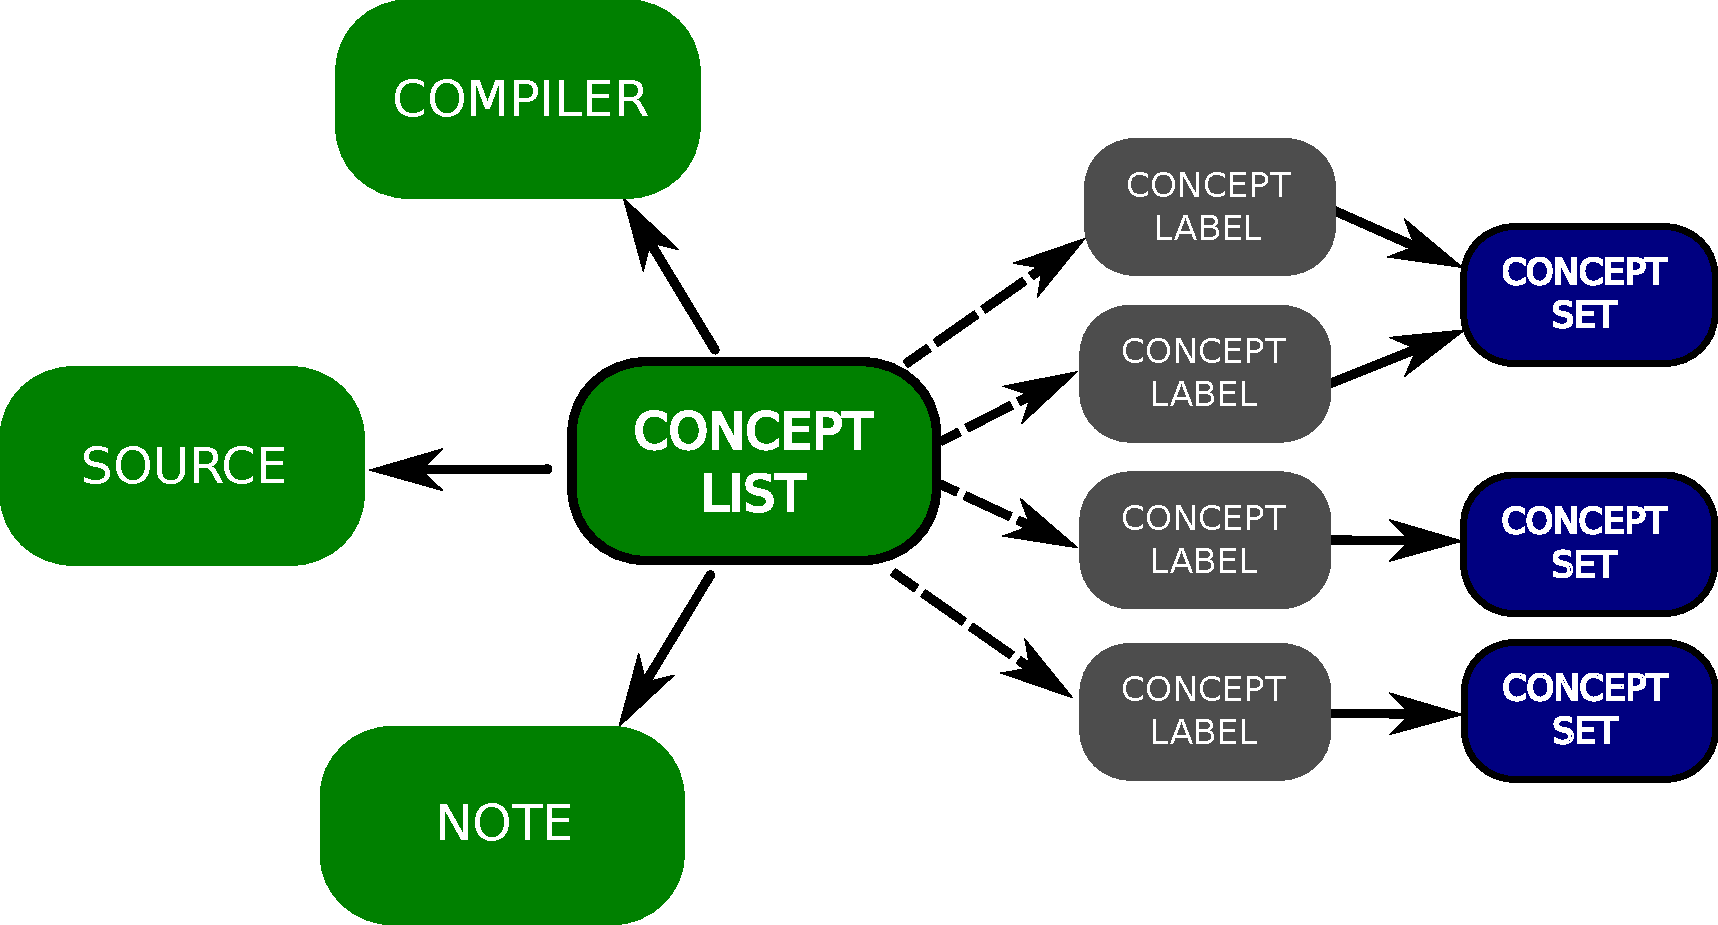
\includegraphics[width=0.475\textwidth]{img/concepticon.pdf}
  \caption{The core data model of the Concepticon.}
  \label{fig:concepticon}
\end{figure}



\section{Examples}
\subsection{CHILD: ``Young Human" or "Descendant"?}
As a first example for both the problems one faces when trying to link concepts across concept lists and the way we
try to address them in the Concepticon, consider the different concept labels for ``child" given in
Table \ref{tab:child}. As we can see from the labels themselves, the label ``child" can denote two
different concepts, of which one could be specified as ``child (young human)" and the other as
``child (descendant)". Not all concept lists, however, offer this precision. Swadesh himself, for
example, would specify the ``descendant" reading in his first list from 1950, but the ``young human"
reading in the list from 1952. In the list by \newcite{Comrie1977}, which was intended to be a merger of
the Swadesh's 200-item list from 1952 and his 100-item list from 1955, this specification is lost,
and we cannot tell from the concept label which reading was intended by the compiler. The same
applies for the lists of Blust (published in Greenhill et al., 2008) and \newcite{Chen1996}.  In order to handle
these problems resulting from ambiguous concept labels, we assign those concepts whose reading we
cannot determine from the concept label and the further descriptions given in the concept lists to a
broader concept set ``CHILD". Additionally, we set up a relation that states that ``CHILD" is both
broader as ``CHILD (YOUNG HUMAN)" and ``CHILD (DESCENDANT)". Figure \ref{fig:child} shows the
relations involving ``CHILD" which have been currently defined in the Concepticon.
 
\begin{table}[h]
  \resizebox{0.475\textwidth}{!}{%
  \tabular{|p{3cm}|p{4cm}|p{3cm}|}\hline
    \bf Compiler                 & \bf CONCEPT LABEL                                          & \bf Concepticon   \\\hline\hline
    Blust                   (2008)       & child                                                 & CHILD                         \\\hline
    Chén                    (1996)       & 孩子 / child                                          & CHILD                         \\\hline
    Comrie and Smith (1977) & child & CHILD \\\hline
    %Dunn                    (2012)       & child                                                 & CHILD                         \\\hline
    Leibniz                 (1768)       & infans                                                & CHILD (YOUNG HUMAN) \\\hline
    Matisoff                (1978)       & child/son                                             & CHILD (DESCENDANT) \\\hline
    Swadesh                 (1950)       & child (son or daughter)                               & CHILD (DESCENDANT) \\\hline
    Swadesh                 (1952)       & child (young person rather than as relationship term) & CHILD (YOUNG HUMAN) \\\hline
    %Tadmor                  (2009)       & child (kin term)                                      & CHILD (DESCENDANT) \\\hline
    %Wiktionary              (2003)       & child (a youth)                                       & CHILD (YOUNG HUMAN) \\\hline
    \endtabular}

  \caption{Concept Labels and Concept Sets for ``child".}\nocite{Greenhill2008}
  
  \label{tab:child}
\end{table}

\begin{figure}[h]
  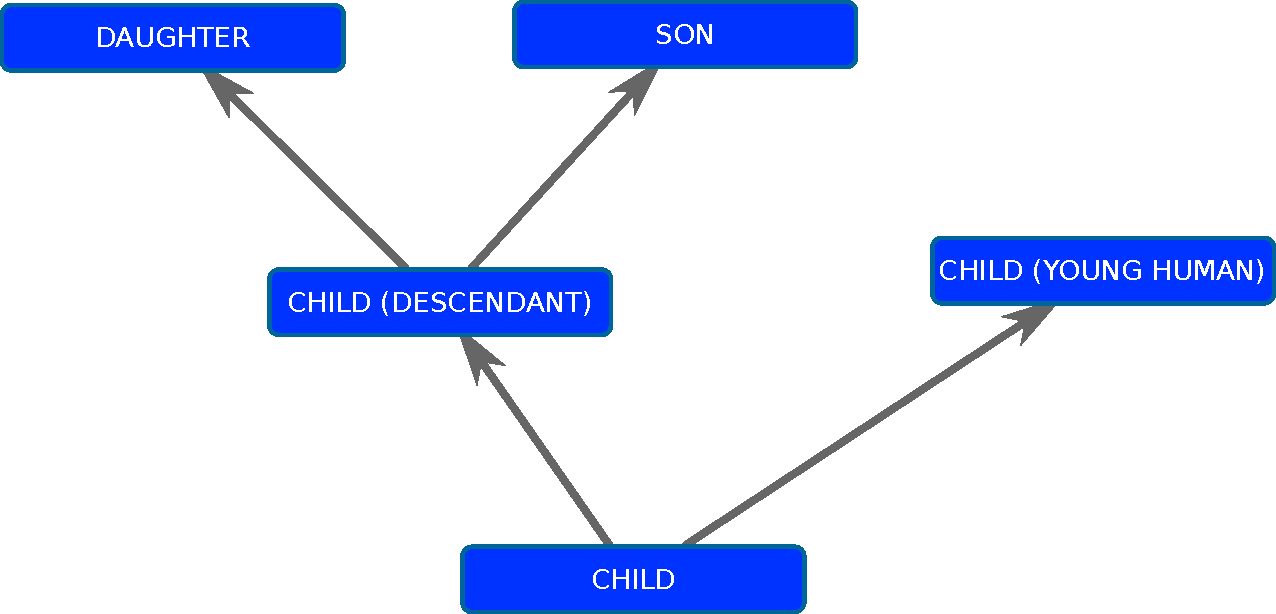
\includegraphics[width=0.475\textwidth]{img/child.pdf}
  \caption{Concept Relations for ``child''.}
  \label{fig:child}
\end{figure}
\subsection{RAIN: Thing or Action?}
Another example for problems involving concept labels in concept lists are basic words related to
``rain". Here, as illustrated in Table \ref{tab:rain}, the problem of mapping is not to find out which reading is intended, since ``rain"
itself is a rather clearcut concept, but it is not possible in all cases to tell whether the
compilers intended to denote the \emph{thing} or the \emph{action}. This is a problem resulting from
the use of English as a language for concept labels, since both the noun and the verb are
homophones. In the lists of \newcite{Leibniz1768} and \newcite{Chen1996}, there is no doubt that the
\emph{thing}-reading is intended, since noun and verb of ``rain" are not homophone, neither in
Chinese, nor in Latin. The same holds for the list by Blust (2008), since it structures the concepts
into specific semantic fields which clearly indicate which reading is intended. In the lists of
\newcite{Swadesh1950} and \newcite{Comrie1977}, however, it is not possible to determine the
intended reading. For this reason, we set up an overarching concept set ``RAINING OR RAIN" which we define as
being broader as ``RAIN (PRECIPATION)" and "RAIN (RAINING)" (see Figure \ref{fig:rain}).

\begin{table}[h]
  \resizebox{0.475\textwidth}{!}{%
  \tabular{|p{3cm}|p{4cm}|p{3cm}|}\hline
    \bf Compiler                 & \bf CONCEPT LABEL                                          & \bf Concepticon   \\\hline\hline
    Blust        2008       &  rain             & RAIN (PRECIPATION)\\\hline
    Chen         1996       & 雨 / rain & RAIN (PRECIPATION) \\\hline
    Comrie and Smith (1977) & rain & RAINING OR RAIN \\\hline
    Leibniz      1768       & pluvia           & RAIN (PRECIPATION) \\\hline
    Matisoff     1978       & rain             & RAIN (PRECIPATION) \\\hline
    Swadesh      1950       & rain                & RAINING OR RAIN\\\hline
    Swadesh      1952       & to rain                                & RAINING \\\hline
    \endtabular}
    \caption{Concept Labels for ``rain"}
    \label{tab:rain}
  \end{table}

  \begin{figure}[h]
  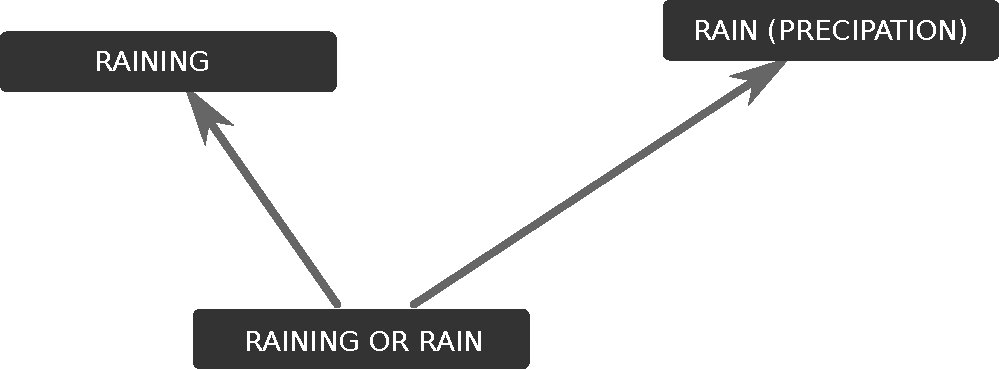
\includegraphics[width=0.475\textwidth]{img/rain.pdf}
  \caption{Concept Relations for ``rain''.}
  \label{fig:rain}
\end{figure}

\subsection{``DULL" or ``STUPID"?}

As a last example for typical problems involving the linking of concept list, consider the concepts
given in Table \ref{tab:dull}. Here, the four lists apparently intend to denote the same concept
``dull". From the Chinese terms used in the lists by \newcite{Wang2006} and \newcite{Chen1996},
however, we can clearly see that the intended meaning is not ``dull" in the sense of ``being blunt
(of a knife)", but ``stupid". Given that both authors originally wanted to render Swadesh's original
concept lists in their research, this shows that we are dealing with a translation error here which
may well result from the fact that in many concept lists, only ``dull" is used as a concept label,
without further specification. 
 
\begin{table}[h]
  \resizebox{0.475\textwidth}{!}{%
  \tabular{|p{3cm}|p{4cm}|p{3cm}|}\hline
    \bf Compiler        & \bf CONCEPT LABEL             & \bf Concepticon   \\\hline\hline
    Blust                 (2008) & dull, blunt                 & DULL\\\hline
    Ch\'en (1996)                  & 呆,笨 / dull       & STUPID\\\hline
    Comrie and Smith (1977) & dull & DULL \\\hline
    Wang (2006)                  & 笨(不聪明) / dull & STUPID \\\hline
    Swadesh               1952 & dull (knife)                & DULL \\\hline
    \endtabular}
    \caption{Erroneous Translations in Concept Lists.}
    \label{tab:dull}
  \end{table}

\section{Using the Concepticon}
\textcolor{red}{HIer eventuell zeigen, wie das Concepticon bei Dictionaria und Lexibank benutzt
werden kann}

\section{Outlook}
\textcolor{red}{heir noch mal sagen, dass wir natürlich noch weiter daran arbeiten.}



\free
\bibliographystyle{lrec2014}
\scriptsize
\bibliography{concepticon}

\end{document}

